
\documentclass{article}[12pt]
%Required: You must have these
\usepackage{graphicx}
\usepackage{tabularx}
\usepackage{natbib}
%\usepackage{caption}
%\usepackage{subcaption}
\usepackage{array}
\usepackage{amsmath}
%\usepackage[backend=bibtex]{biblatex}
\setkeys{Gin}{width=0.8\textwidth}
%\setlength{\captionmargin}{30pt}
\setlength{\abovecaptionskip}{10pt}
\setlength{\belowcaptionskip}{10pt}
\topmargin -1.5cm 
\oddsidemargin -0.04cm 
\evensidemargin -0.04cm 
\textwidth 16.59cm
\textheight 23.94cm 
\parskip 7.2pt 
\renewcommand{\baselinestretch}{1.1} 	
\parindent 0pt

\bibliographystyle{refs/styles/newphyto.bst}
\usepackage{Sweave}
\begin{document}
\Sconcordance{concordance:prief_outline.tex:prief_outline.Rnw:%
1 2 1 1 0 47 1}


\section{Introduction}
\begin{itemize}
\item Phenology, the timing of seasonal life cycle events such as leafout, seed germination etc, is important for lots of things, especially species interactions, and helps give rise to the rich community biodiversity we observe today.
\item Phenology is shifting due to climate change, but shifts vary among species.
\item These shifts are sure to affect interactions altering patterns of competition/coexistence, but exactly how is unknown, because eco-physiological underpinnings of phenology are not yet well integrated with models of long-term community dynamics.
\item This limits our ability to forecast community change and manage the biodiversity crisis.
\item First, we provide empirical about germination phenology and environmental cues to demonstrate how phenological differences contribute to community coexistence and how phenological sensitivity---differences in \emp{how} species respond to climate variation----alters these differences. Then we adapted a common model of community dynamics (often conceptualized for two competing species of plants with a seedbank) to explicitly model the timing of germination over the season depending on winter climate conditions to assess how the tradeoff between phenological sensitivity and competitive ability changes under alternate climate conditions. Finally, we provide some future directions.

\item \textbf{probably need to specify we are talking competition/same trophic level, and maybe in general be more specific about limiting the scope of our inquiry}
\end{itemize}
\section*{How phenology mediates species interactions/competition}
\begin{itemize}
\item Phenological differences among competitive species can serve as a stabilizing mechanism (define) between species.
\item By being active at different times increases strength of intraspecific vs. inter specific competition. Also serves as a seasonal priority effect- allowing earlier species a head start, niche modification etc.
\item If superior competitors are also earlier active the can rapidly exclude competitors. ie this is what we think some invaders do. Priority effects can can allow weaker competitive to exclude stronger ones (Figure 1).

\item Priority effects can lead to coxistience if the weaker competitor is earlier, and the difference in phenology is proportionate the the difference in competitive ability. For example, we found that the two species we studies had an average overall phenological differences of appx. 7 days (Fig 2a). Therefore, assuming a specific (slope) of the relationship, they would coexist if there difference in competitive ability was X (Fig 2b).

\item However, phenological timing is not an intrinsic species trait---in most ecological systems, phenology is strongly controlled by climate cues (e.g., temperature, light and moisture) making phenological differences among taxa the variable product of an interaction between species’ unique sensitivity to environmental variation and the annual environmental conditions they encounter. Considering phenology sensitivity is key to understanding the efffects of climate change on coexistence.
\end{itemize}

\section*{How phenology sensitivty mediates phenological differences}
\begin{itemize}
\item Temperature, light, moisture cue phenology, but species respond differntly to these cues. 
\item In general, higher levels not only advance spring phenology, but also reduce differences amoung species.
\item This is apparent in our germination study (Figure 3a). 
\item This is the tricky part to describe: This suggest the differences in competitive ability necessary for coexistence are conditioned on (evolved?) long term climate patterns. For example if community received on average 12 weeks of chilling phenological differences between aster and smart weed would be X, but in lower chill (6 weeks), it would be Y (Fig 3b). This is impossible (assuming here R*s are an intrinsic species traits). This suggest species that coexist under one climate condition will not be able to if the average climate conditions shift. You'd need a species with different sensitivty to produce the same phenological differences.
\item But how while this relationship between sensitivity and competition shift?
\end{itemize}
\section*{Predicting the tradeoff under climate change}
\begin{itemize}
\item All these things, are hard to observe (germination, competition, coexistence) and experiments are limited in the timescale in their ability to link them. But combining empirical experiments with models can allow to get a better sense of this.
\item Plagiarized from my esa abstract: We adapted a common model of community dynamics (often conceptualized for two competing species of plants with a seedbank) to explicitly model the timing of germination over the season depending on winter climate conditions (Methods S1). We parameterized this model based on estimates of phenological sensitivity to environmental variation from a series of germination assays performed with herbaceous plant species of eastern temperate forests. By running our simulations under both contemporary and future (warmer) conditions, we were able to parse how the phenology-competition tradeoff of coexistence is likely to shift with climate change. 

\item Under both high and low chill scenarios, the relationship between phenolgical differences and competition was the same (as expected).  However, these relationship between phenological sensitivity and competition shifted. The slope got steeper and coexistence less frequent with lower chilling (Fig. \ref{Fig:coexistence}). 

\item Why you might ask? As we saw indicated in the case study above with aster and smart weed, under high chilling, species tended to germination at the same time (Fig 4b), but under lower chilling the same sensitivity differences resulted in larger phenological differences (Fig 4a,b).

\item Some speculative implications in real communities? Increased diversity of physiological mechanisms that affect sensitivity. For example, communities with different kinds of dormancy, or ones that use different cues. Phylogenetically more diverse?

\item But there are some step we probably need in order to actually begin to understand this.
\end{itemize}

\section{A path forward}

Our model is only the beginning, and while it is a noteworthy advance worthy of being published in a nature subsidiary or equivalently high impact journal, there is still a long way to go to forcast these dynamics. Here are some critical aspects.
\textbf{I think I need help here. All of my thoughts are pretty germination/chilling specific. I could use some idea for contextualizing this more broadly in phenology, and coexistence}
\begin{enumerate}
\item Germination phenology as a response curve. We do a good job of modeling quantitative responses to forcing and water potential. Bad job for stratification of seeds, which is super critical in alot of parts of the work.
\item Longer term. Experiments with seasonal cary-over. Most SPE studies only apply the priority effect once. When in reality, communities reassemble each season.
\item Seasonal priory effects and other germination variation. In this study we were super focused on phenology so we held germination \% steady. Future model extension could include both.
\end{enumerate}



%Even co-occurring (plant) species with similar growth forms, habitat requirements and environmental tolerances often express markedly different phenologies. These differences in phenology are an important mediator of competition \citep{}, allowing early-active species to access limited seasonal resources and modify the growth environment before competitors emerge \citep{Kardol2013},These phenological differences serve as a stabilizing (or equalizing? I always get them confused) mechanisms between species with different intrinsic competitive abilities (i.e., weaker competitors germinate first).


%\item \textbf{Baby:} This tradeoff between phenology and competitive ability is plays a major role in community coexistence, 

%\item \textbf{Wereworlf:} In most (temperate?) regions of the world, phenology is strongly controlled by climate cues. Climate is changing, and phenology is too, though we see huge differences in how species respond to climate. This suggest that climate change will disrupt the patterns of coexistence and restructure communities.

%\item \textbf{Wereworlf cont.:} Understanding how climate change will alter this fundamental tradeoff between phenology and competition is critical for forecasting community change, which has implications for conservation, restoration and management. Unfortunate we are limited in our ability to do this.

%\item While we have good understanding of the eco-physiology of phenological variation, the role of seasonal priority effects (differences in within-season arrival timing among species) in competition, and sophisticated models of coexistence, these areas aren't well integrated, so we are limited.

%\item We know the physical environment (temperature (forcing and chilling), light, and moisture) exert strong control over the relative timing of germination, vegetative growth and reproduction, but most of our empirical evidence about how phenological difference effect competition come from germination studies using sequential planting studies, that do not incorporate the mechanism of environmental control. 

%\item We know asymmetric responses to environmental variation is a critical aspect of coexistence, models of coexistence have not broadly integrated phenology module, and cannot differentiate between phenology influence and the seed bank dynamics. \textit{Not sure how true this is, and if we want to go here or not}

%\item \textbf{Silver bullet:} Integrating environmental experiments with models that bridge this gap is key.  Here we: %using examples from empirical germination assays we then used sexy, 
%1) use examples from empirical germination assays to address fundamental questions about the how differences in phenological sensitivity to the environment manifest different realized patterns of phenology under varying environments.
%2) Integrate these patterns into a coexistence model to assess how the tradeoff between phenological sensitivity and competitive ability changes under alternate climate conditions.
%3) Provide future directions.

%\item Seasonal priority effects, may play an important role in maintaining species coexistence,. At an the extreme, precocious germination could also allow weaker competitors to competitively exclude stronger ones--- a trait which of often invoked to explain the success of invasive plants, many of which germinate rapidly and early in the growing season \citep{Gioria2018,Gioria:2017wo}.

%\item Phenology is strongly linked to climate. We've seen big changes but responses vary among species. This suggest that SPEs will change too, and their resulting patterns of coexistence too, but can't predict this 

%\item Why not. Most of our experiments don't factor in climate at all. Plus they are too short.


%\section*{Seasonal Priorty Effects are dependent on seasonal environmental variation}
%\begin{itemize}
%\item In most ecological systems, the timing of seed germination is under strong environmental control \citep{}. In arid ecosystems water and temperature matters \citep{}. In other temperate and boreal systems, chilling matters. Species vary in there sensitivity to the factors \citep{}. These factors also vary \citep{}. Therefore the phenological differences among species that generate seasonal priority effects are the manifestation of the interaction between sensitivity to the environment (which varies among co-occurring species) and the environment itself. This means that interannual variation in environment strongly influences the strength of the seasonal priority effects.

%\item To better understand these dynamics, we performed a series of germination assays with regionally co-occuring herbaceous species under varying chilling and incubation conditions. We used these studies to estimate species level sensitives to these environmental cues, and forecast phenological differences among species under difference climate conditions (see Supplemental Methods.)

%\item From these trials we see three things. 
%\begin{enumerate}
%\item Species have different sensitivities to the same cues (Fig. \ref{Fig:emp}. This was true for species with the same dormancy class, closely related species and those in the same habitat (Make Supplemental figure.)

%\item In general, at higher levels of chilling, the sensitivity differences reduced the realized differenences in germination phenology amoung species and lower levels increased them. (Fig. \ref{Fig:surv}). Incubation temperature were interesting because species cross the the optimum (Fig. \ref{Fig:emp}), which also made it that cooler temps standardize phenology (Fig. \ref{Fig:surv}). \textit{Lizzie, we've talked about this being a phenomonon observed more broadly, do you know citations for this?}

%\item One thing this means is that species with similar and different sensitives can express different and similar phenology. For example the species in Fig. \ref{Fig:case}. (I'd potentially like to develop this into a ``box" with pretty pictures of the species, some statements about how they might compete---e.g. Dames rocket is an invasive species that can invade meadows where it would compete with milkweed and forest edges where it would compete with jumpseed.).
%\end{enumerate}

%\item This also give us insight about the tradeoff between competetion and phenology. Under a stable environment coexistence could be achieved through a trade off. If that shifts, the trade off should shift. 

%\end{itemize}

%\section{Models to the rescue}
%\begin{itemize}
%\item Models can define sensitivity and competitive ability. Can isolate germination phenology from other germination responses and simulate long term dynamics and environmental change. We modified a model to coexistence to do this.

%\item  Genreal paragraph about our model with ref to Supplement

%\end{itemize}
%but this is hard to study .Of course the biggest challenge is we cannot observe coexistence. Explain the experiments, most experiments manipulate the SPE directly by sequential planting, that means even in experiments last for multiple seasons, the priority effect is only applied once (decide where to talk about this). Other unrealism of this approach discussed in our previous paper.

%The tradeoff between competition and phenology is hard to measure. Models that link all these things can help.
%Even isolating the phenological sensitivity is lacking. Most germination studies dont fit curves, just biany or threshhold effects.
%Species have different sensitivity to environmental cues (Fig 1a), which manifests in different patterns of phenological assembly under different conditions, species with similar sensitivies can manifest strongly different effects under some conditions, and species with different sensitives can converge. This mean 
%A second complexity is germination phenology isnt the only aspect the at dependent on the environment. The number of seeds that germination affect this dynamics too. Complexisty

%\section{Coexistice and competitive exclusion under alternative climate scenario}
%\begin{itemize}


%Cases where the stronger competitor (lower Rstar) was extripated due to phenological differences also occured in both scenario0s. Slope didn't change, but the frequency did.

%\item Fig. \ref{Fig:differences} explains both of these phenomena. Mainly germination differences are minimized when chilling is met \ref{Fig:differences} a). And the relationship between sensitivity differences and realized phenology differences changes \ref{Fig:differences} a).

%\item Need some help thinking through Fig. \ref{Fig:coexistence} b). Why does frequency of weaker invader winning increase. My guess is just that phenological differences are bigger more often, so the magnitude of the priority effects are bigger. 
%\end{itemize}


\pagebreak
\section*{Figures}
\begin{figure}[h!]
  \centering
 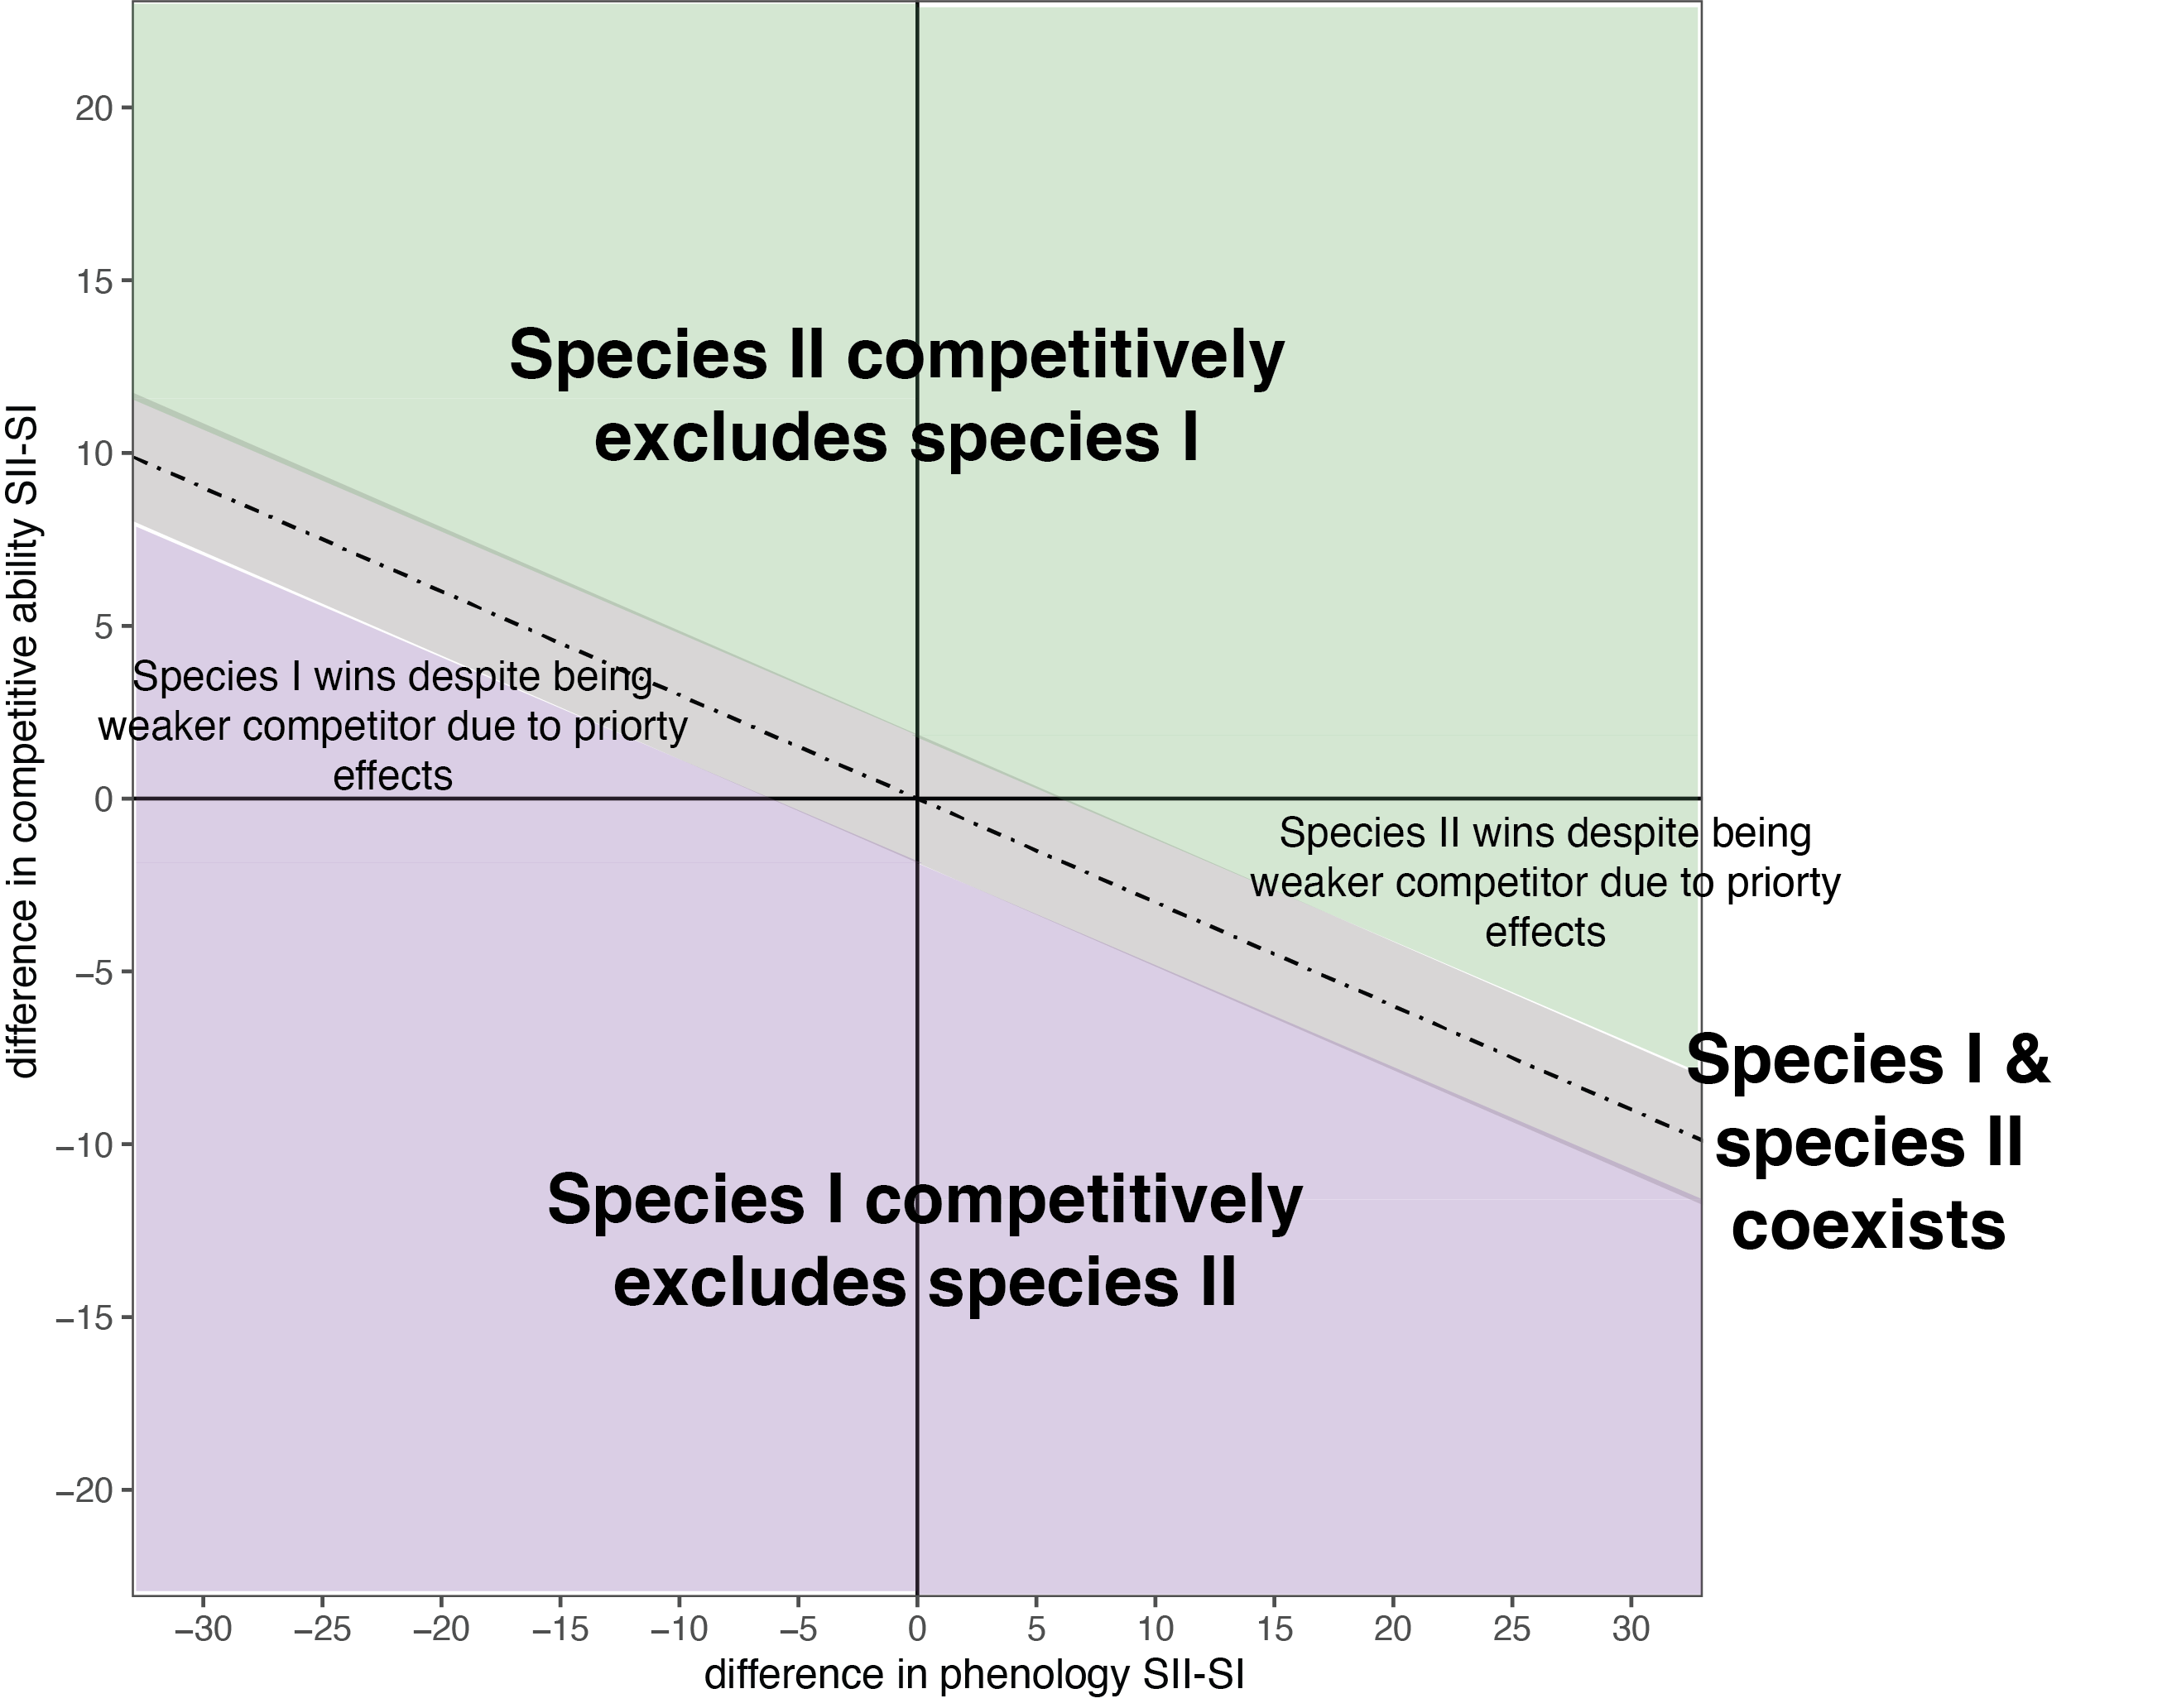
\includegraphics[width=\textwidth]{..//plots/introprief.png}
    \caption{Concept}
    \label{Fig:con1}
\end{figure}


\begin{figure}[h!]
  \centering
 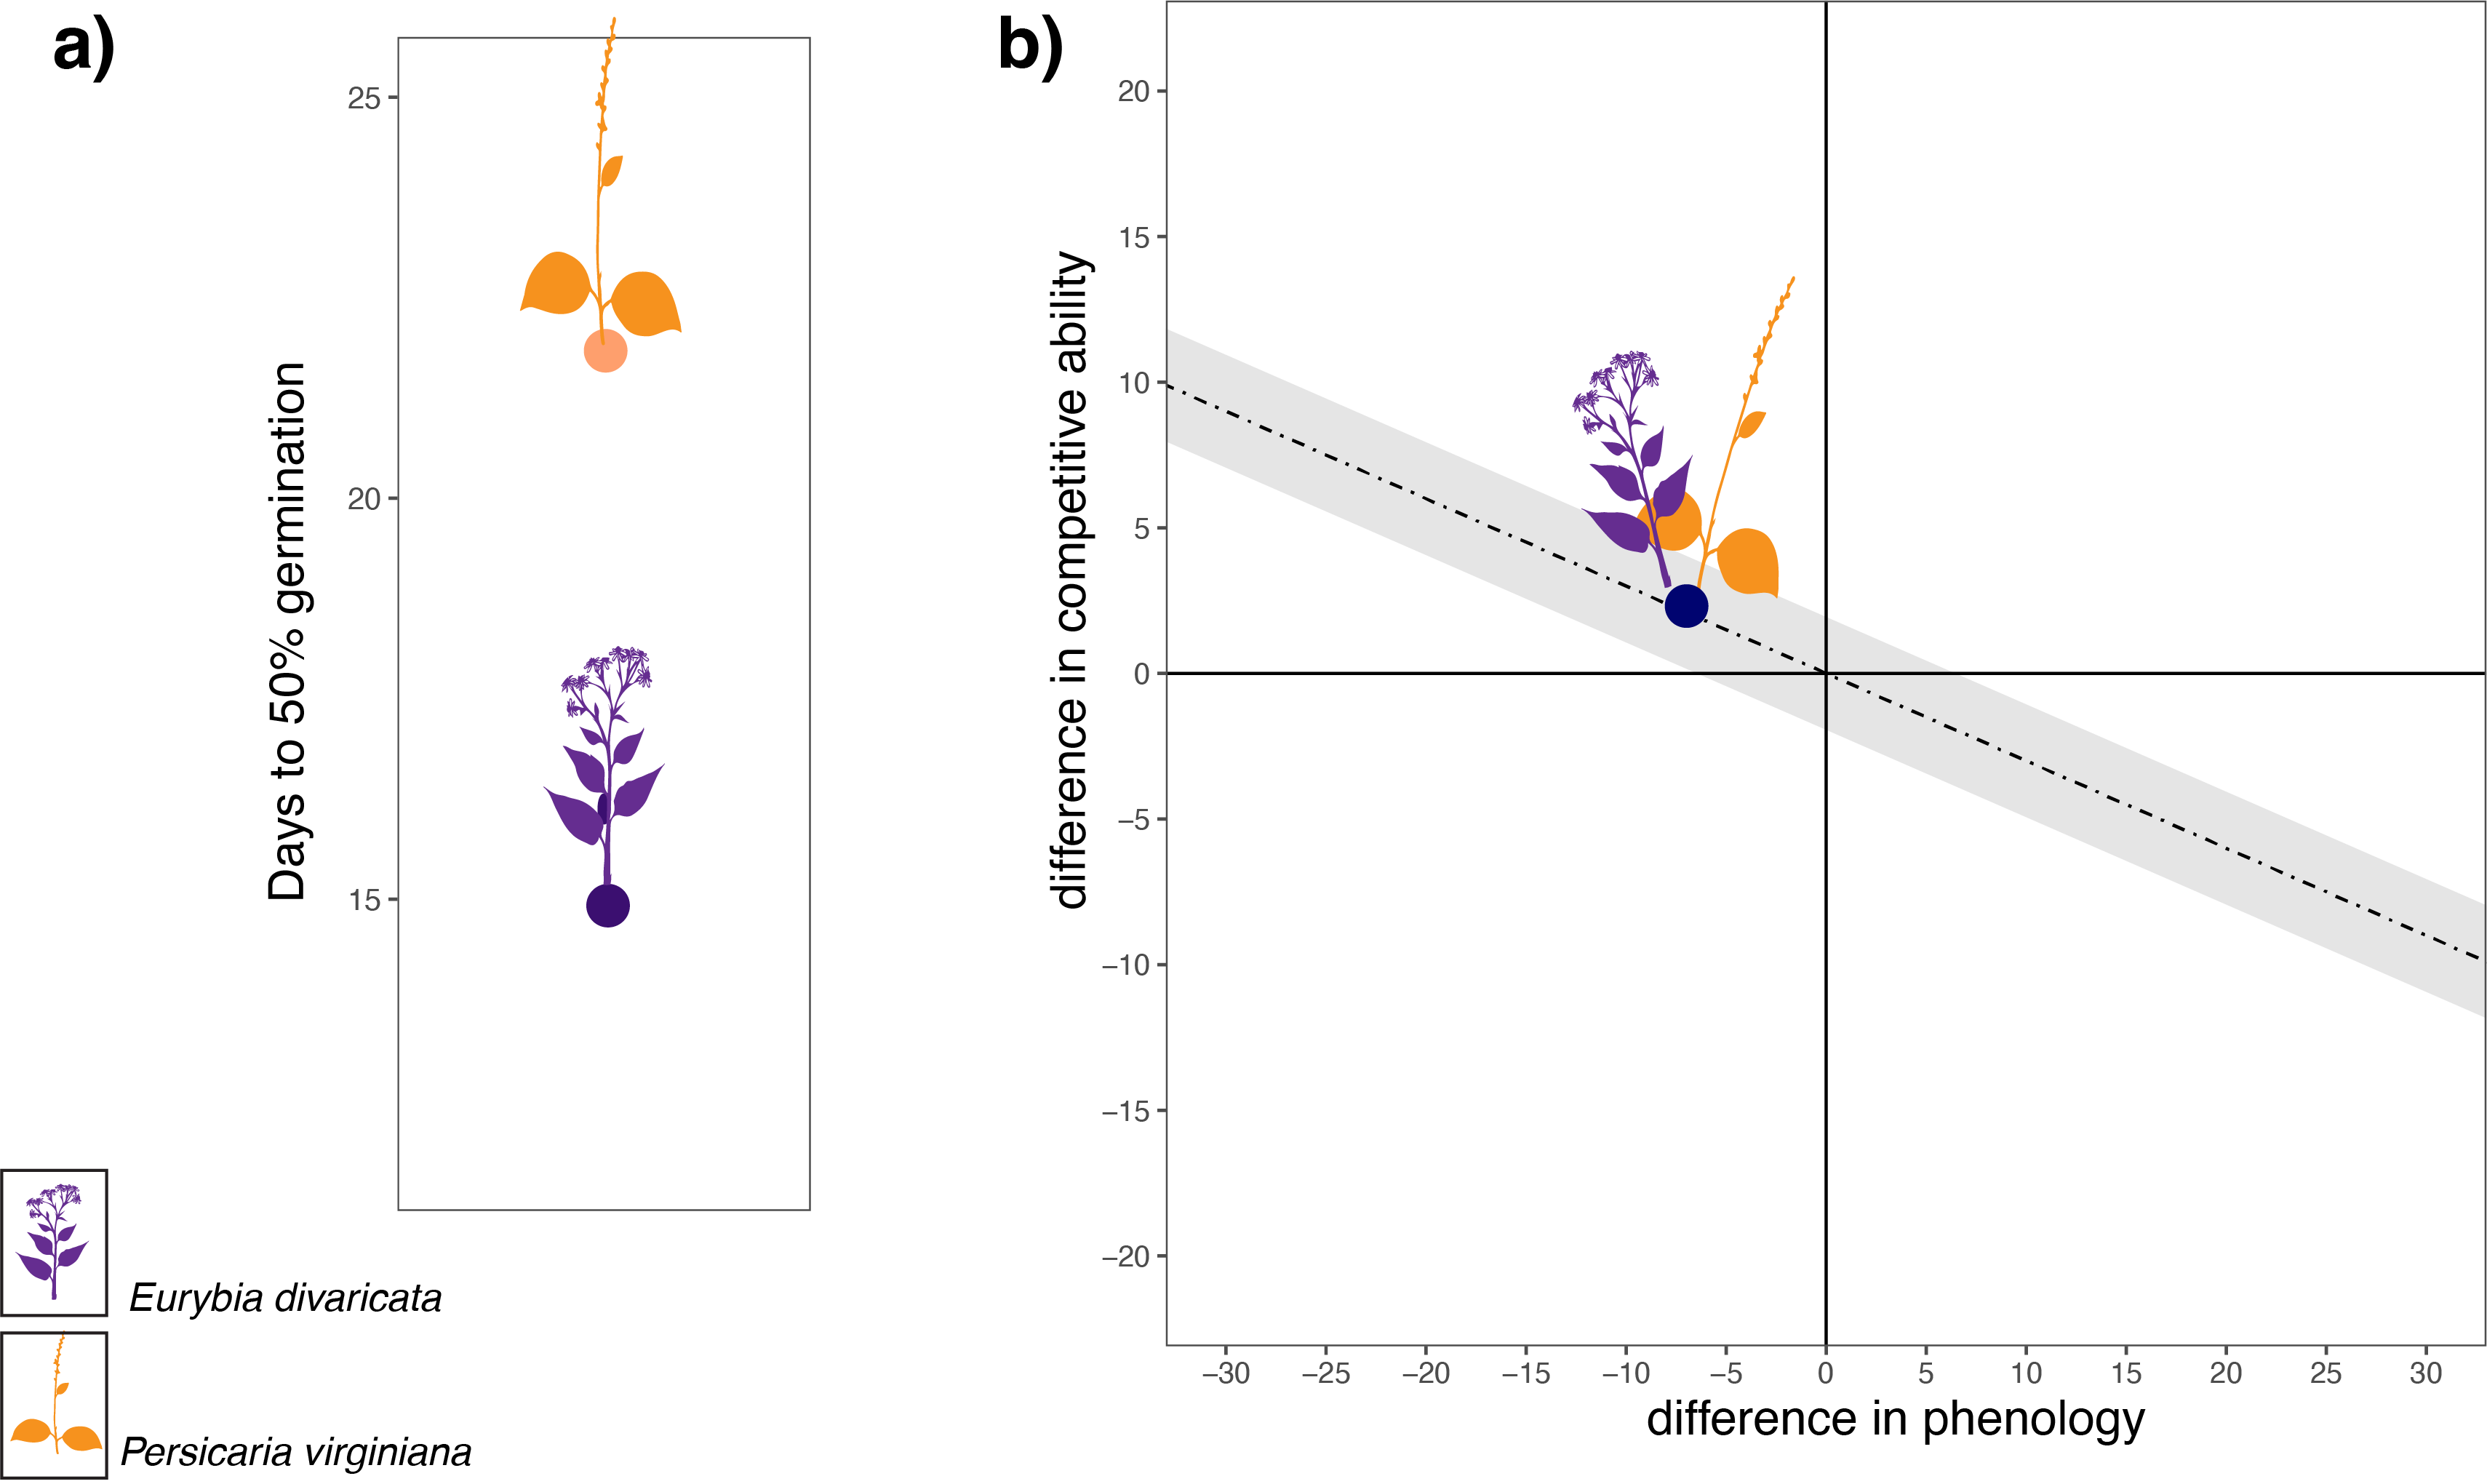
\includegraphics[width=\textwidth]{..//plots/prief_meangerm.png}
    \caption{}
    \label{Fig:means}
\end{figure}


\begin{figure}[h!]
  \centering
 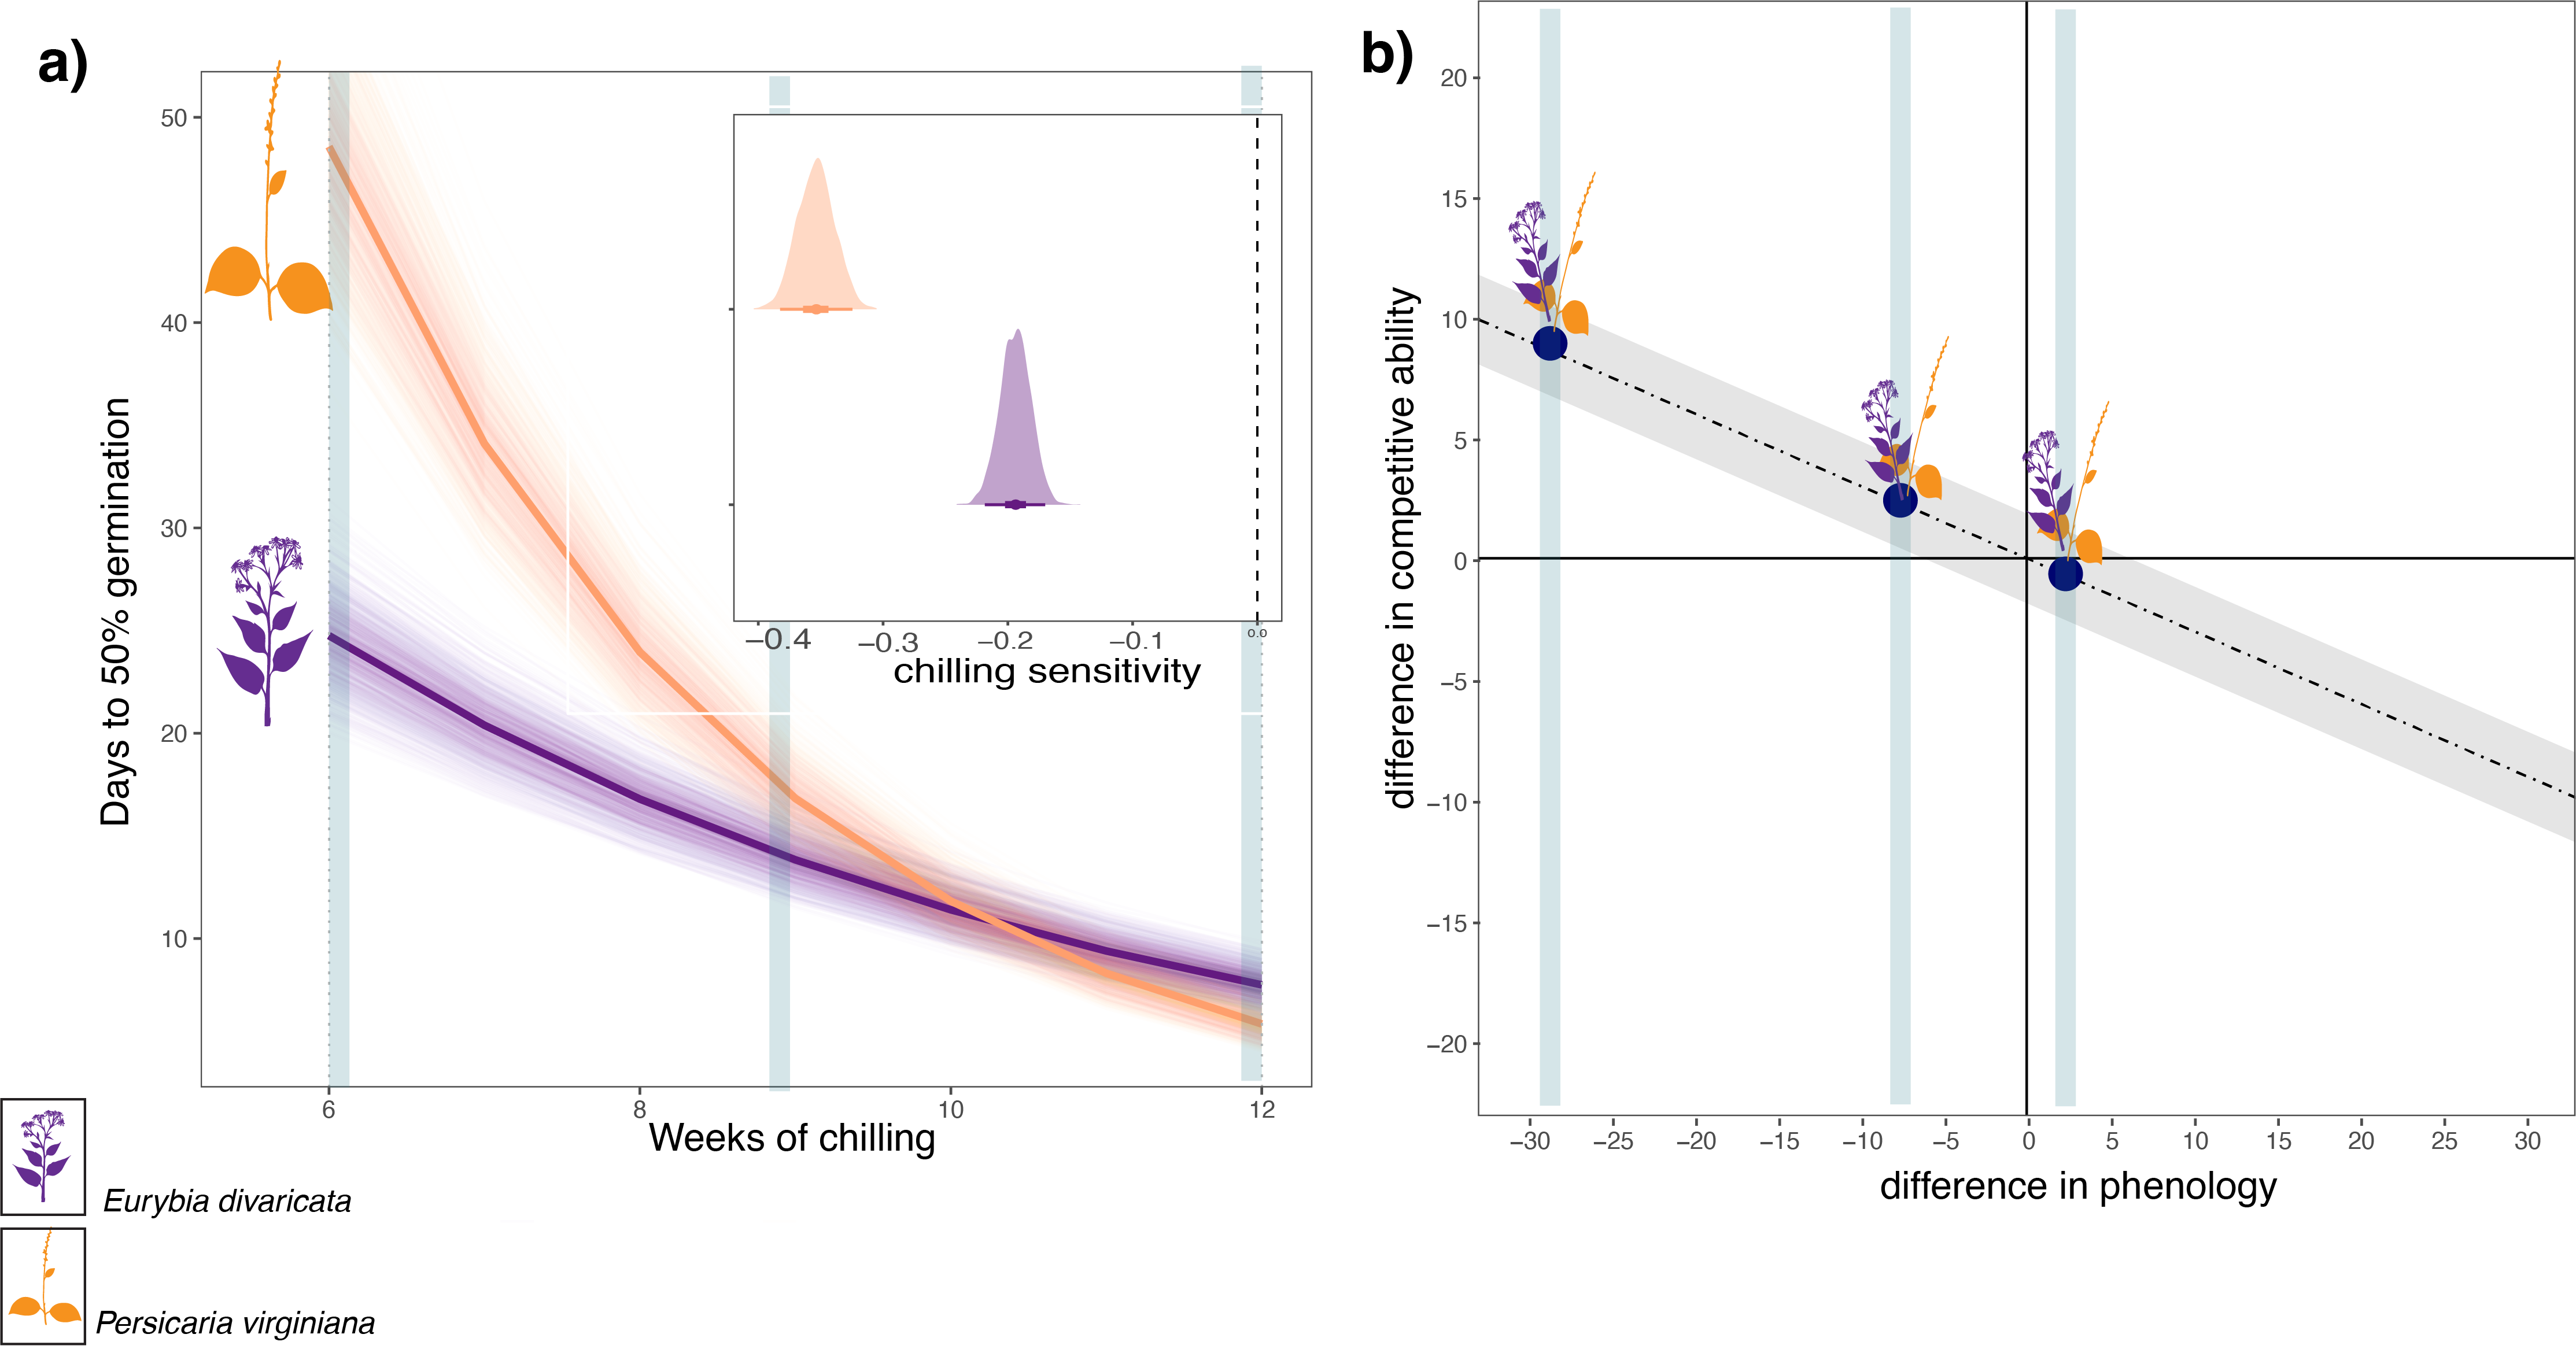
\includegraphics[width=\textwidth]{..//plots/prief_sense.png}
    \caption{}
    \label{Fig:sensy}
\end{figure}


\begin{figure}[h!]
  \centering
 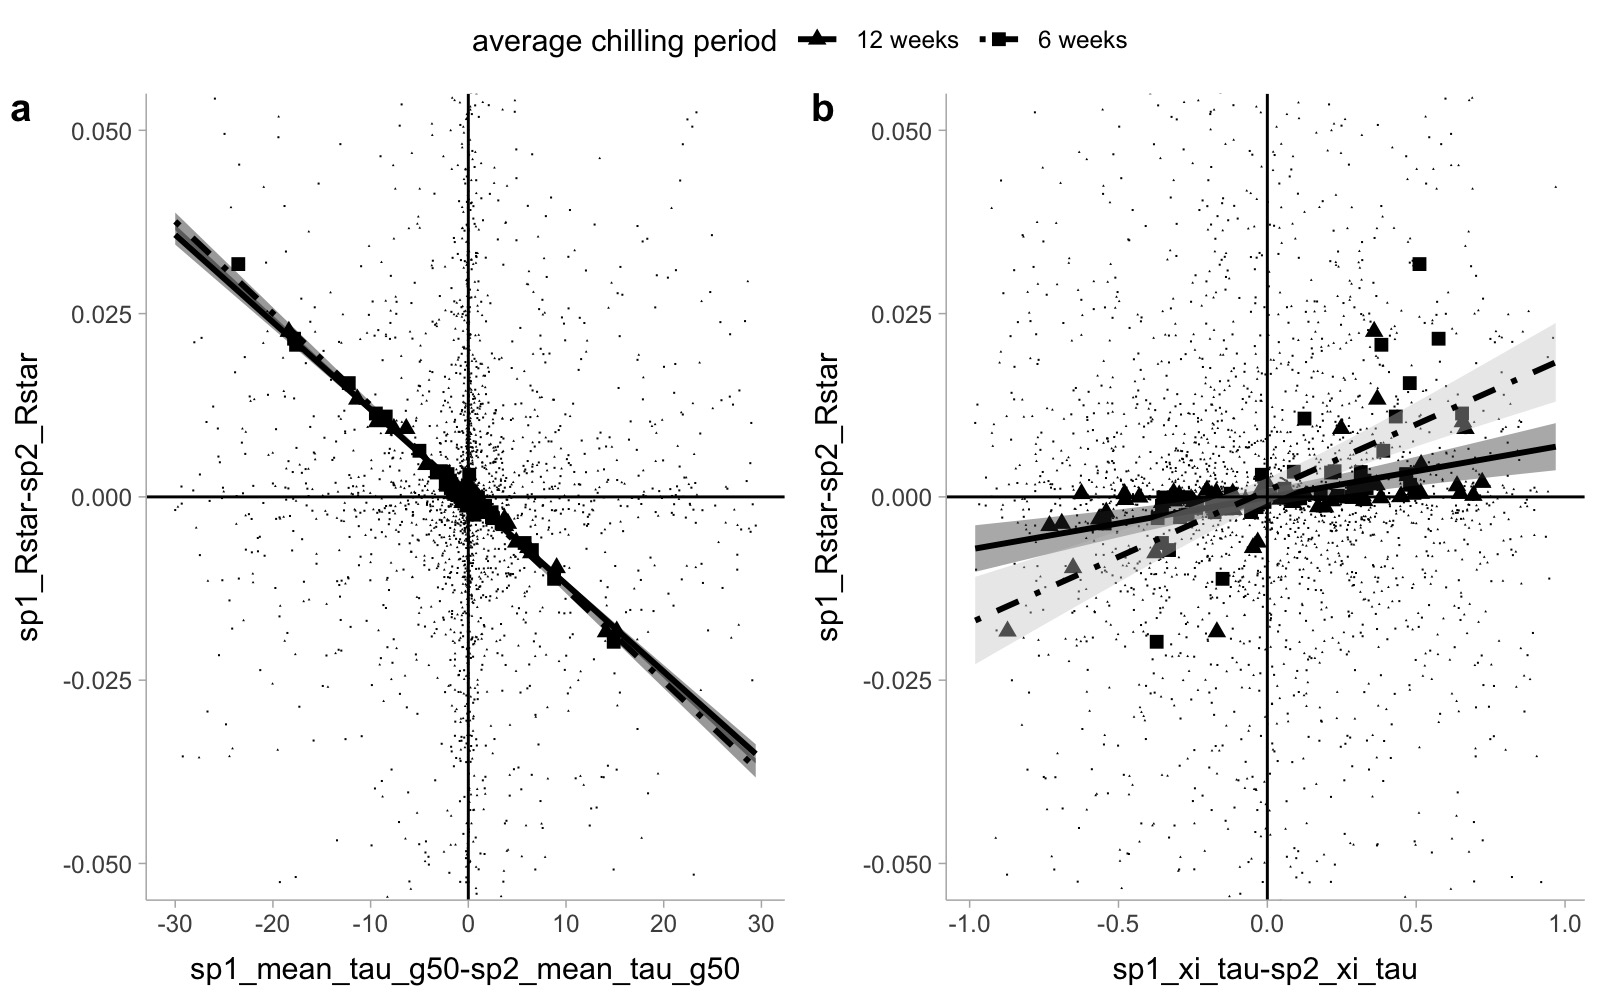
\includegraphics[width=\textwidth]{..//plots/coexistance_runner_new.jpeg}
    \caption{}
    \label{Fig:coexistence}
\end{figure}


\begin{figure}[h!]
  \centering
 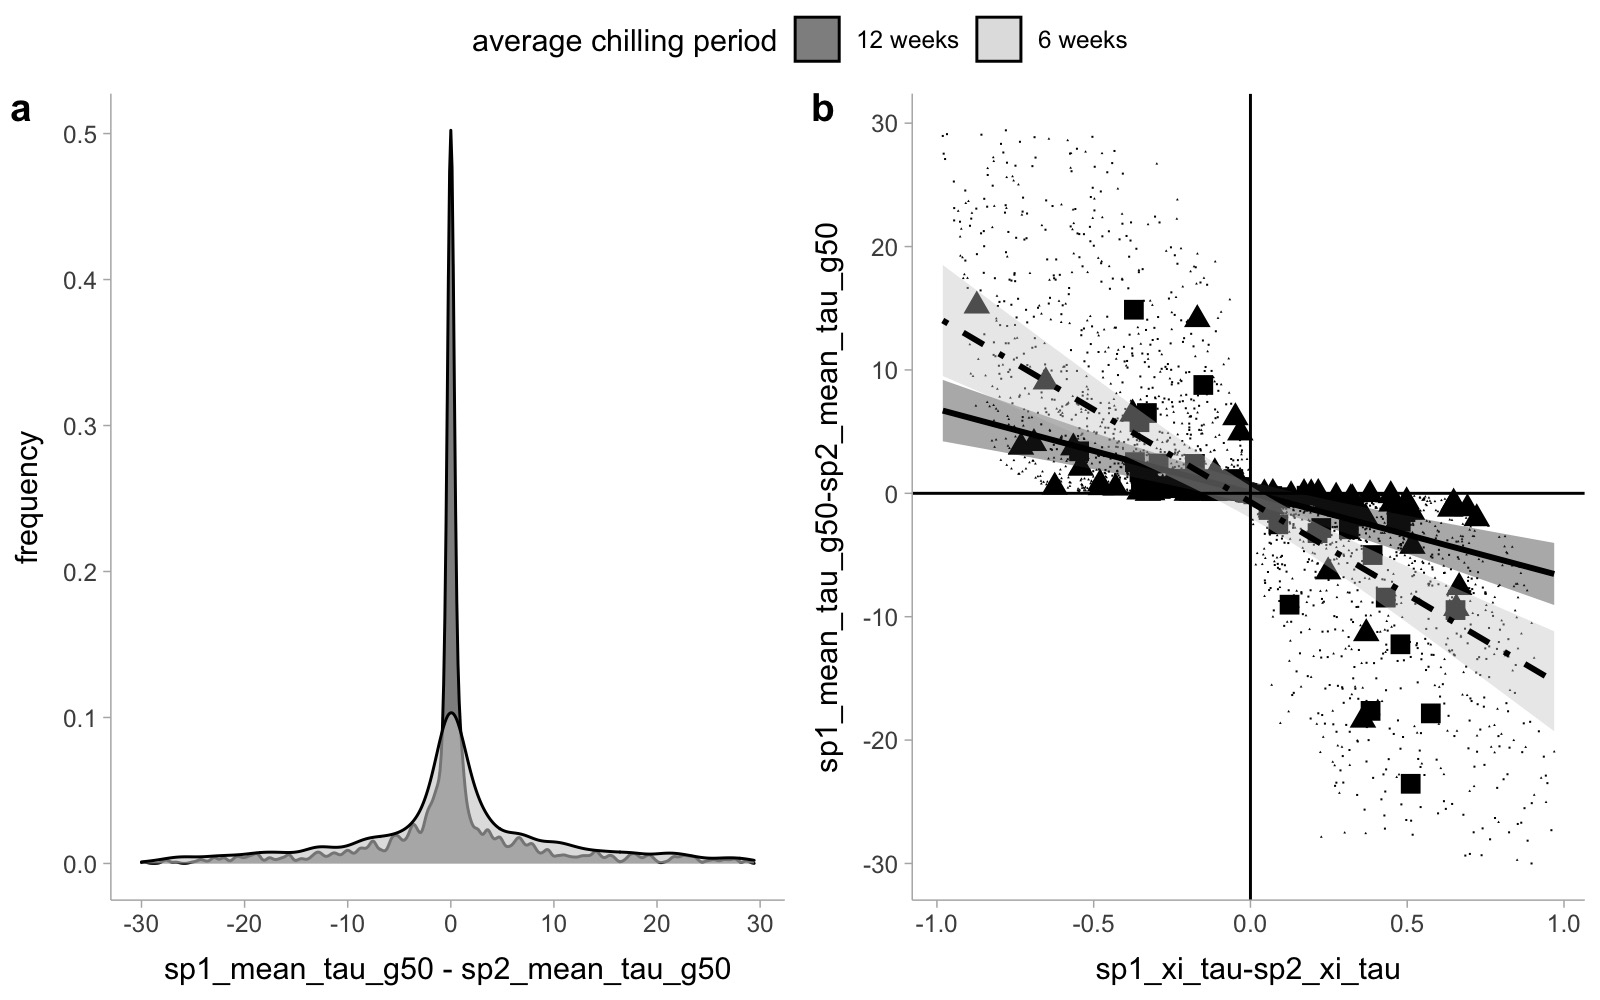
\includegraphics[width=\textwidth]{..//plots/coexistance_explainer.jpeg}
    \caption{}
    \label{Fig:differences}
\end{figure}


\end{document}
